\chapter{绪论}
%
	第十四届全国人民代表大会第三次会议通过的政府工作报告进一步强调,要加速推进人工智能与实体经济的深度融合,实施“人工智能+”战略进而构建具有全球竞争力的数字产业集群,通过数字化转型推动经济高质量的发展,从而达到提升人民生活质量\cite{China2025}的目的。在这一背景之下机器人导航的研究与应用迎来了新的发展机遇。随着人工智能技术的不断进步和应用场景的深化,机器人目标物体导航\cite{zhang2022survey}作为机器人与人工智能交叉领域的关键技术持续受到学术界和产业界的高度关注。多模态融合的导航技术近年来在自动驾驶、智能家居、服务机器人等领域取得了显著进展\cite{majumdar2022zson},尤其是在复杂和动态环境中的应用潜力得到了广泛认可。尽管技术持续不断的突破,已知环境下的机器人导航仍然面临诸多挑战。本文聚焦于已知室内环境中的目标物体导航问题\cite{sun2024survey},这一场景对传统视觉导航方法提出了更高的要求。传统方法通常依赖于预先构建的环境地图来实现机器人的定位与路径规划,但在复杂多样且动态变化的室内环境中,无法十分有效地完成导航至目标半米内的任务\cite{mavrogiannis2023core}。同时,基于语言视觉的导航方法仅依赖于视觉图像获取环境信息,无法充分利用环境中的感知信息高效地完成导航任务\cite{li2023reinforcement}。

	本文针对室内已知环境下的多模态融合导航方法的研究及实现这一主题提出了一种语言视觉激光多模态融合的机器人导航方法,并将该方法在真实的移动机器人上进行部署,搭建成了一套已知环境下的机器人视觉导航系统。本章的主要内容包括:室内已知环境下语言视觉激光多模态融合导航方法的研究背景和意义、国内外研究现状、研究内容和论文组织架构。

\section{研究背景和意义}
	随着我国经济的快速增长和平价经济时代的到来,物流运输、仓库存储和酒店等各行各业都在寻找能够实现缩减人工成本的同时提高工作效率和精确性的新兴技术手段。
	而移动机器人凭借其安全性高、灵活性好、效率突出等优势逐渐成为这些行业中的重要工具\cite{reddy2023advancements},例如用于物流仓储的自动化搬运机器人、农业领域的智能喷洒设备以及医疗环境中的自主消毒装置等,如图\ref{serverrobot}。
	即使应用领域不断地扩展和变化,自主导航能力仍然是移动机器人实现位置变更和环境交互的基础,是其完成特定多样化任务需求的核心技术支撑随着这一技术的不断发展,机器人研究社区衍生出许多针对不同的场景下不同的室内已知环境导航方法来实现这种自主导航技术。这种技术主要分为激光雷达导航\cite{zhang2014loam}和视觉导航\cite{kazerouni2022survey}两种方法。
	\begin{figure}[htbp]
		\centering
		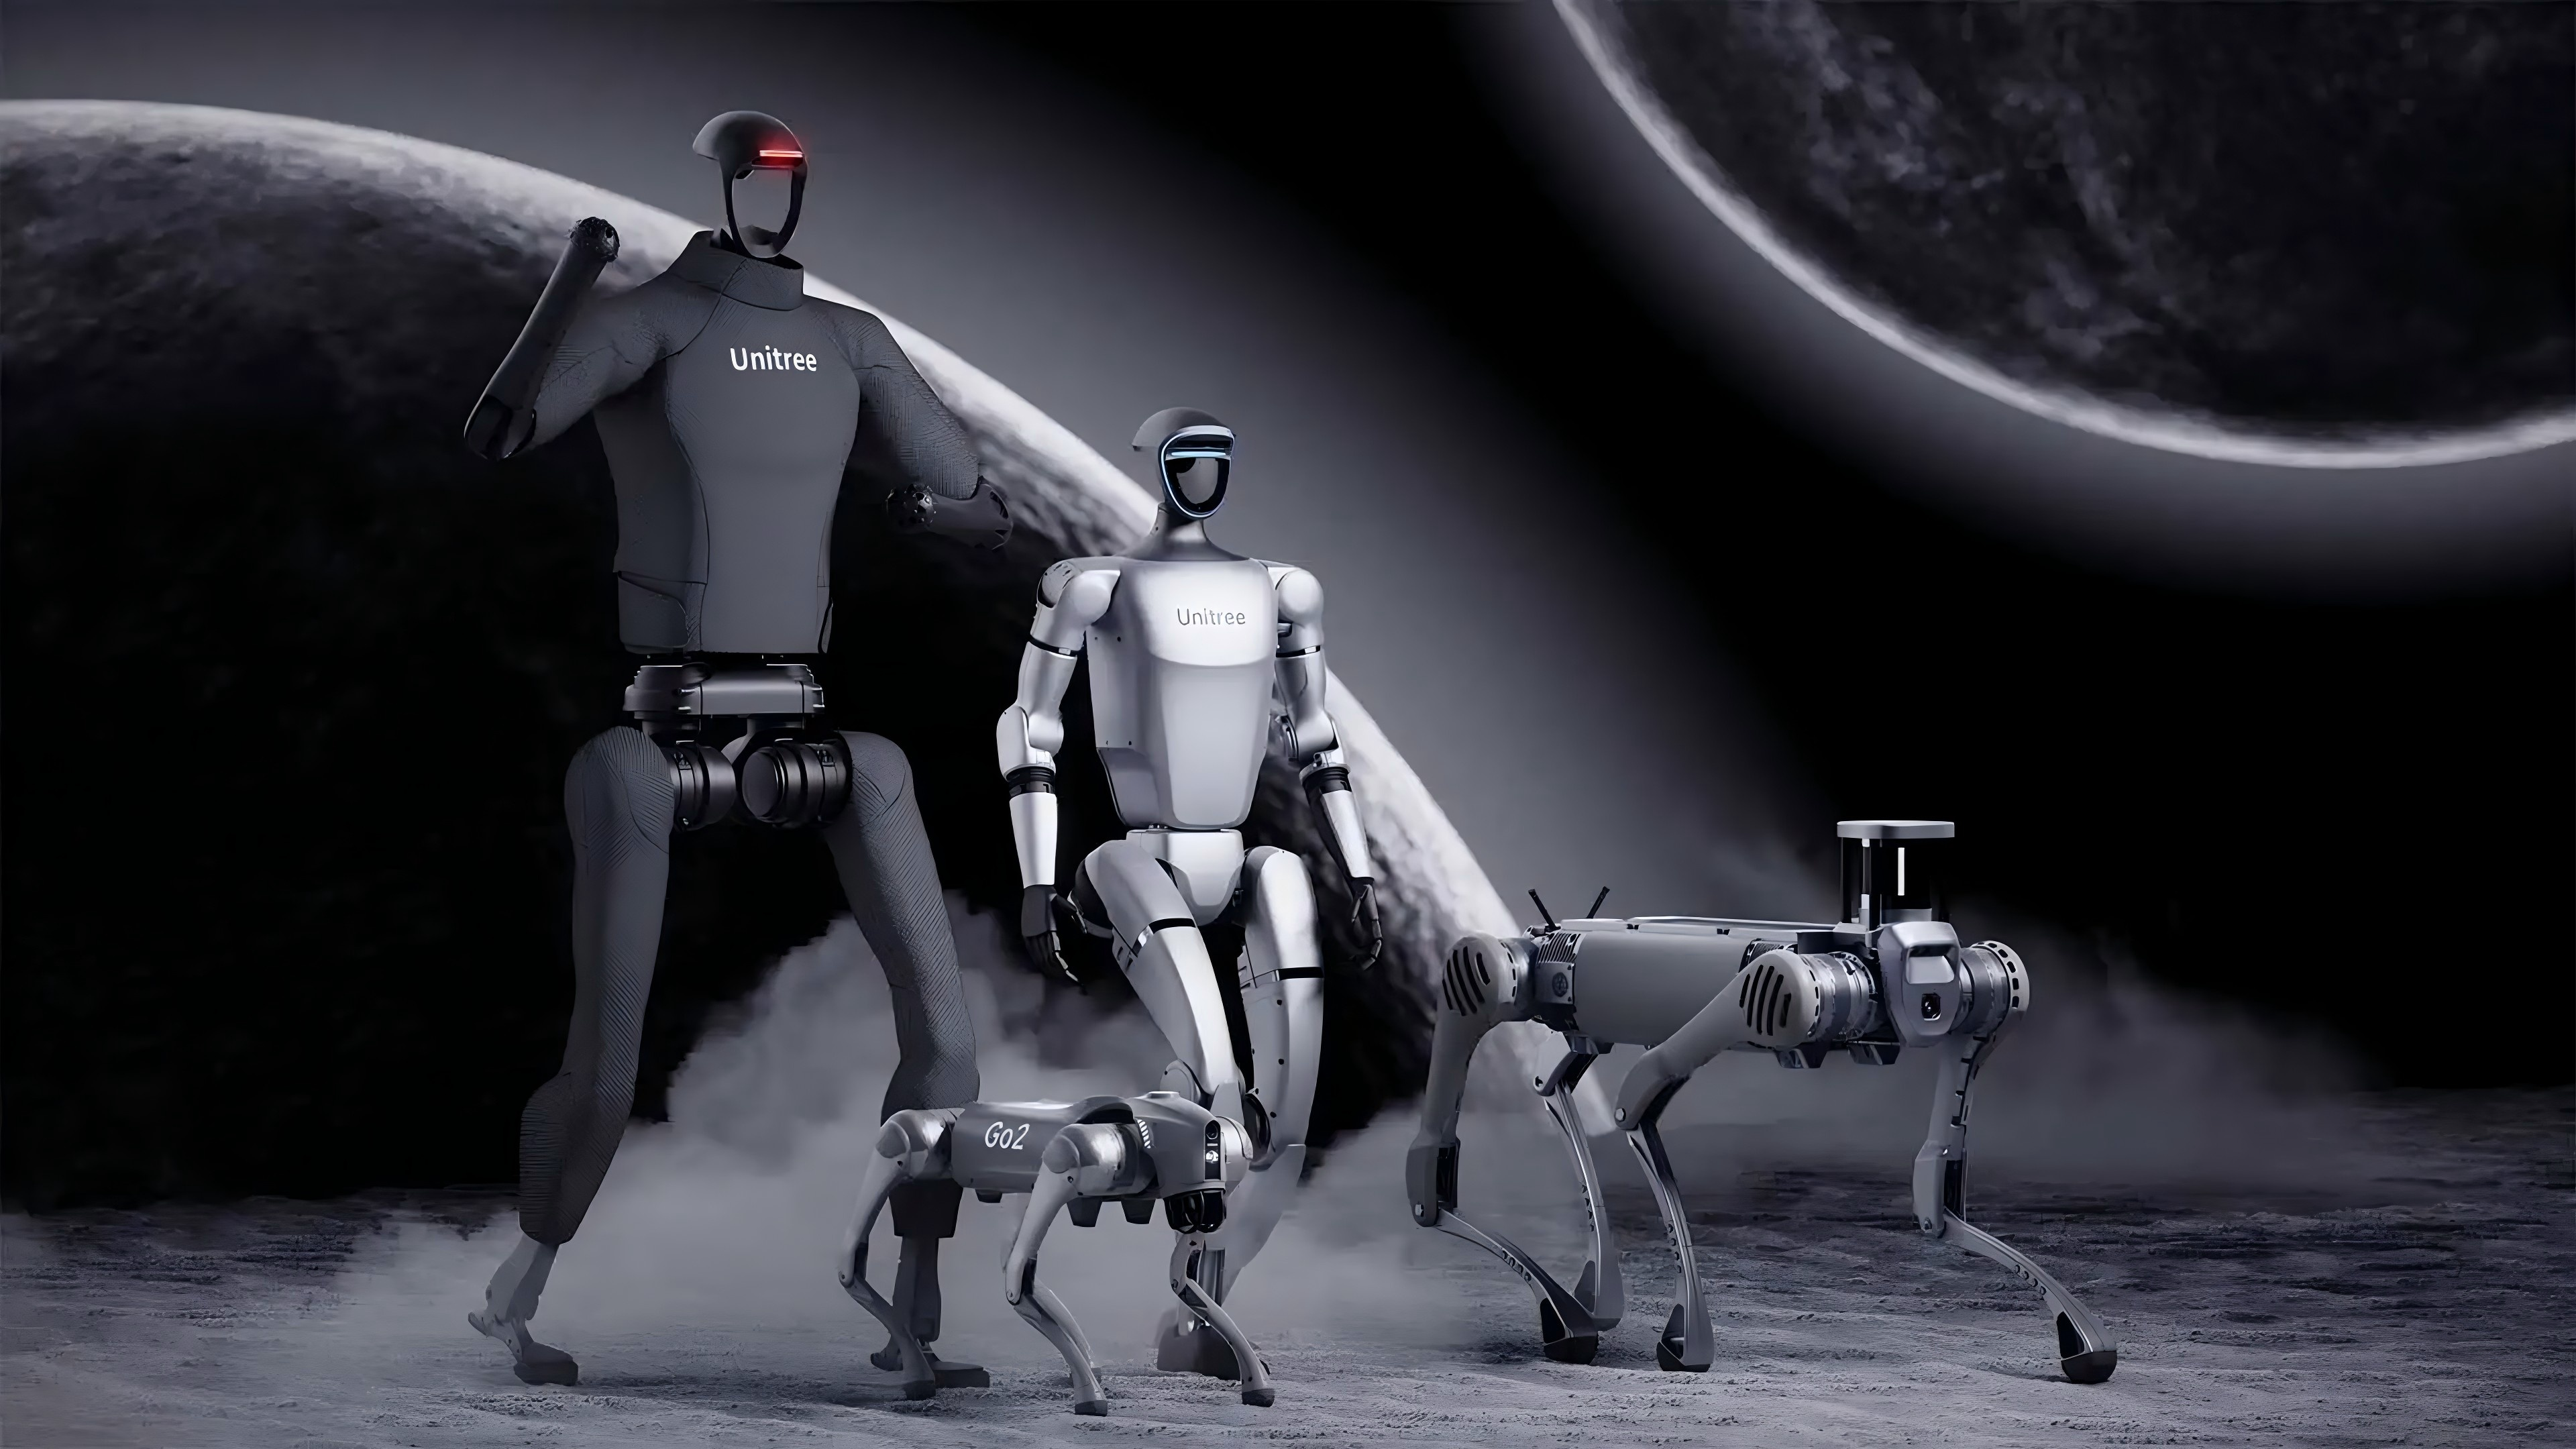
\includegraphics[scale=0.10]{Fig/yushuRobot.png}
		\caption{\label{serverrobot}多功能服务机器人}
	\end{figure}

	
	早期的自主导航技术主要依赖于激光雷达来实现,其完整的导航系统整合了多个领域的算法。目前大多数的机器人研究都基于机器人操作系统ROS\cite{ROS2018}进行开发,其导航框架通常包括以下步骤:利用实时定位与建图(Simultaneous Localization and Mapping,SLAM)\cite{dellaert1999monte, thrun2001robust}技术,激光雷达通过旋转式激光发射装置获取平面障碍物的精确距离信息,使移动机器人能够在未知环境中实时构建环境地图并同步确定自身所处的空间位姿,接着通过如A*算法\cite{hart1968formal}这类全局路径规划算法在所构建的栅格地图中生成全局路径,为了让移动机器人在变化的环境中避免碰撞的同时尽可能沿着生成的全局路径行驶,大多数机器人都采用时间弹性带(Timed Elastic Band,TEB)算法\cite{rosmann2013efficient}作为其局部路径规划算法进行导航,最终抵达目标点。
	这种预先构建精确栅格地图的传统的导航方法在静态环境中表现良好,但在动态环境中却显得力不从心。此外,这类方法难以处理视觉和语义等富含特征的信息,极大地限制了其应用范围。

	人工智能技术的快速更新迭代使得机器能够通过深度学习实现对特定目标的识别与理解,这类技术赋予机器从海量数据中自主学习的能力而无需依赖人工干预。它不仅能够处理可以存储在关系数据库中的结构化数据,还能高效地分析和学习例如文本、图像和音频等这类非结构化数据,得益于深度学习这些方法的强大的学习能力,使其已在众多任务中展现出卓越的性能。人工智能算法在推荐搜索、语音识别与翻译、语义分割、目标检测等领域等典型的应用场景任务中的准确性和效率甚至超越了人类水平。总的来说这种基于深度学习模型的视觉导航方法在动态复杂多变的环境中表现良好,但这种方法无法充分利用环境中的感知信息可靠且高效地完成导航任务,其在静态环境中的导航准确率和导航效率不如传统依赖于激光的导航方法。

	上述的这些问题都制约了室内服务机器人的发展,我们急需找到一种能够动态调整以适应静态环境和复杂多变环境的导航方法。激光雷达导航方法具有更为完整的开发社区,它能利用激光雷达的感知信息预先构建精确栅格地图,并在实时导航的过程中可靠地避障并导航至目标点。在这个过程中仍存在着部分的难题。首先,需要读取并提取自然语言指令中的关键信息。其次,需要设计一种多模态融合网络,提取环境中获取的感知特征、认知特征、指令语义特征和地图特征以获得潜在的目标点的概率。最后,还需要利用指令中可能存在的方位信息设计一种方位优化算法,以提高导航的成功率。同时,由于激光雷达导航方法依赖于地图导航点的设置,无法适应于多变的环境,无法导航至目标半米内。因此还需要设计一种视觉导航方法。首先,需要设计适用于视觉导航的深度学习网络结构,以提高导航的成功率和效率。其次,必须提高模型对未知环境的适应性以提供一定的探索能力。最后,还需解决如何将训练好的模型部署到计算受限的真实机器人上的问题。
	综上所提出的所有问题,本文致力于语言视觉激光多模态融合的导航方法,旨在提出一套有效的室内目标物体导航方法并应用于真实机器人,使其具备类似人类的全局性和灵活性。这将有助于解决机器人在复杂多变环境下的导航需求,推动机器人产业的发展。

\section{国内外研究现状}
    针对不同的传感器和应用场景,目标物体导航可以分为基于SLAM的导航和视觉语言导航。基于SLAM的导航是指利用激光雷达或摄像头预先在环境中创建好栅格地图,在地图中标记各导航点并利用简单的拓扑信息和目标信息实现导航。它通常应用于环境变动不大的场景,如仓储物流中的自动引导机器人、工业自动化中的生产线物料运输机器人、酒店迎宾送餐机器人等。视觉语言导航是指利用摄像头和其他传感器并借助计算机视觉技术,在环境中实现自主导航、自主避障的过程。这种导航常用于车辆导航、行人导航或地图服务中。此外,随着实体机器人在各行各业的需求不断扩大,强调智能体的感知、决策与行动都必须通过自身与环境的动态交互来实现的具身智能逐渐从理论转向了实践。

\subsection{基于SLAM技术的导航方法}
	
	根据感知设备的不同SLAM技术可以划分为基于激光雷达和基于视觉传感器的两大技术路线。利用激光雷达进行环境感知与建图的技术体系的发展历程较视觉方案更为长远。在卡尔曼滤波理论的发展过程中研究者们先后提出了扩展型和无损型两种改进算法,这两种算法在当时迅速成为SLAM领域的主流解决方案。其中扩展型卡尔曼滤波在实际应用中存在一定局限性,它不仅需要预先确定运动轨迹,并且在系统模型和噪声统计特性不明确的情况下还可能出现算法不收敛这种致命问题。


	Murphy\cite{murphy2001rao}等人在Rao-Blackwellised粒子滤波中引入状态变量边缘化技术,有效缩减状态空间维度并提升采样效率。然而这种方案存在计算资源消耗过大的问题,在复杂特征的场景下会对SLAM算法的实时性造成负面影响。
	为了解决上述问题,Grisetti\cite{grisetti2005improving, grisetti2007improved}等人进一步优化了RBPF框架并提出了Gmapping算法。该算法通过融合机器人运动学模型与局部观测数据,从而显著降低了位姿预测的不确定性。此外,其改进的重采样策略有效缓解了粒子退化的现象,使该方法成为激光SLAM领域兼具鲁棒性和实用性的代表性解决方案。
	后来,Cartographer\cite{hess2016real}和LSD-SLAM\cite{engel2014lsd}这类基于图优化的SLAM解决方案采用前后端分离的架构设计,其中,前端模块负责处理机器人位姿的实时更新,后端模块则专注于全局位姿与环境特征的联合优化,二者协同工作构成了完整的SLAM系统。这种架构虽然在复杂场景下具有较高的建图精度,但在计算效率方面存在一定局限。
	Zhang\cite{zhang2017low}等人将SLAM这一复杂问题划分成两种算法,一种以高频但低保真度执行里程计,另一种以低频但高保真度用于点云的精细匹配,提出了针对激光点云进行特征提取的激光SLAM系统。
	在轻量级的SLAM算法之中,Shan\cite{shan2018lego}等人开发的LeGO-LOAM算法针对地面场景进行了专门优化。他们的方法通过识别点云数据中的平面和边缘特征求解计算连续扫描间的六维位姿变换,并最终实现了适用于计算受限的嵌入式平台的高效定位方案。
	LO-Net\cite{li2019net}框架创新性地结合了激光雷达与深度学习技术,通过采用端到端训练模式,使移动机器人的位姿预测精度得到显著提升。
	孙海\cite{孙海2017激光测距在仓储搬运机器人运动中的应用}等人为了解决仓储搬运机器人的导航需求,采用基于激光的同步定位与地图构建技术来通过环境中的线性特征提取从而实现了室内地图的构建,该方案不仅解决了仓储环境中的特征识别难题,还推动了激光SLAM技术在实际工程中的应用发展。
	
	基于视觉传感器的SLAM方法主要通过处理图像数据来实现机器人的位置感知,尽管它的研究历史与激光SLAM方法更短,但随着深度学习技术的不断发展也同样取得了显著的技术进展。该技术在状态估计方面主要形成了两种方法论:一种是通过提取图像特征点进行计算,另一种则直接利用图像像素信息进行处理。基于特征点的运动估计方法的核心思想是通过提取图像中的特征点并建立匹配关系,进而推算出机器人的位移和姿态变化。
	Davision\cite{davison2007monoslam, davison2003real}等人提出了一种MonoSLAM系统,通过一种主动地映射方法、测量方法以及单目特征初始化和特征方向估计方法实现了一种能够进行实时定位的纯视觉SLAM系统,它是视觉SLAM方法的起源因此具有里程碑的意义。
	PTAM\cite{klein2007parallel}算法在视觉SLAM领域实现了重要突破,他们首次采用前后端分离的架构设计,并创新性地引入了关键帧机制实现了地图构建与位姿跟踪的并行处理。但该算法在后端优化效率方面存在明显不足,这一局限促使后续研究者在他们成果的基础之上将非线性优化理论作为视觉SLAM的重点研究方向。此后ORB-SLAM\cite{mur2015orb}系统进一步拓展了视觉SLAM的应用范围,可支持单目、双目及深度相机等多种传感器模式,同时还通过引入闭环检测机制显著提升了定位精度。
	直接法视觉SLAM通过原始图像数据直接计算相机运动。LSD-SLAM\cite{newcombe2011dtam}是直接法的经典实现方案,它采用直接处理图像信息的策略而无需特征提取即可完成机器人的位姿估计,通过使用视频流中可用的数百张图像与整个密集模型对齐来精确跟踪相机的运动,在快速运动下具有卓越的跟踪性能。Foster\cite{forster2014svo}等人提出了一种半直接单目视觉里程计(Semi-direct Monocular Visual Odometry, SVO)算法,SVO消除了对昂贵的特征提取和强大的运动估计匹配技术的需求,直接作用于像素强度,使其定位精度和鲁棒性大大提高。





\subsection{视觉语言导航方法}
	Wen\cite{wen2025zero}等人设计了一种基于思维树的视觉语言网络(Visual Language model with a Tree-of-Thought Net, VLTNet),在多路径选择和必要时的回溯时创新性地使用ToT推理框架,能够以更高的准确性做出全局决策,在涉及复杂自然语言作为目标指令的场景中表现出色。
	Unl\cite{unlu2025reliable}等人提出了一种由用于初始检测的GLIP视觉语言模型和用于验证的InstructionBLIP模型组成的双组件框架,解决传统方法对于标记数据的依赖局限,提高模型目标导航过程中的语义理解,从而增强机器人在不熟悉环境中的自主性。
	Alvare\cite{gutierrez2025visual}等人针对视觉语义导航问题提出了一种新的具身代理解决方案,在基于ROS的系统上设计了一种可以兼容视觉语义导航模型(Visual Semantic Navigation Model, VSN-model)的新型导航框架,以便任何的VSN模型都可以轻松部署在任何兼容ROS的机器人中,并在真实的环境中进行测试,以提高具身代理的性能和效率。但这种方法对于不同的VSN解决方法存在着明显的性能差异。
	Yuan\cite{yuan2025exploring}等人提出了一种可以在目标导航任务中进行可靠前沿选择的方法,引入了一种由多元化专家前沿分析(DEFA)和共识决策(CDM)组成二点多专家决策框架,解决基于基础模型的系统中常见的荒谬或不相关的推理,在RoboTHOR和HM3D数据集上都展现了最先进的性能,擅长导航到未经训练的对象或目标。
	Jones\cite{jones2025beyond}等人通过利用自然语言作为通用的跨模态基础,在大数据集不易获得的异构传感器模态上微调视觉运动通用策略,将多模态对比损失与基于感觉的语言生成损失相结合来编码高级语义,提出了能够适用于大型视觉语言动作模型的FuSe导航方法。
	
	Long\cite{long2024discuss}等人引入了一种新颖的视觉语言导航(Visual Language Navigation, VLN)学习框架,使用具有不同能力的大型模型作为领域专家构建了导航代理DiscussNav,在每一步行动之前会通过涵盖指令理解、环境感知和完成度估计在内的专家讨论,用于纠正无意的错误和筛选不一致的运动决策以有效地促进目标导航。
	Zhou\cite{zhou2024navgpt1}等人提出了一种纯粹基于大语言模型(Large Language Models, LLMs)的指令跟踪导航代理NavGPT,可以显示地执行包括将指令分解为子目表、整合与导航任务相关的常识知识、从观察到的场景中识别目标、跟踪导航进度以及通过计划调整来适应异常情况这种导航的高级规划。尽管NavGPT在R2R任务测试过程中的性能仍然低于经过训练的模型,但可以通过调整LLMs的多模态输入和显示推理来优化基于学习的模型。后来他们通过拟合VLN专业模型和基于LLM的导航范式之间的差距,同时保持LLM在生成语言和导航推理方面的解释能力,从而整合了一种优化后的导航代理NavGPT-2\cite{zhou2024navgpt2}来实现有效的动作预测和导航推理。
	Liu\cite{liu2024dragon}等人提出了一种由对话系统DRAGON提供支持的引导机器人,能够将环境与自然语言联系起来。通过理解用户的命令,将用户的自由格式语言与环境相结合,并通过口语为用户提供语义信息,引导用户在地图上找到所需的地标。
    
	2024年,Yokoyama\cite{yokoyama2024vlfm}等人借助人类推理的方式设计了一种视觉语言边界地图(Vision Language Frontier Maps, VLFM)来帮助代理在新环境中导航到新环境中看不见的语义目标。该方法根据观测深度图构建栅格占据地图以确定潜在的导航路线,在通过观测图像和预先训练的视觉语言模型生成基于语言的价值图,并据此来确定最优导航路线。该方法在按照路径长度加权完成对象目标导航任务指标中取得了最先进的结果。
	An\cite{an2024etpnav}等人提出了一种基于拓扑规划导航框架(Evolving Topological Planning Navigation, ETPNav),它利用基于transformer的跨模态规划器根据拓扑图和指令生成导航计划,再通过试错启发式避障控制器执行该计划。
	Guo\cite{electronics11071136}等人借助ROS框架提出了一种有效的目标导航策略EONS,首先对常见的室内物体进行语义关联分析,利用Mask R-CNN和残差连接网络建立物体语义关联模型,通过ROB-SLAM系统方法构建了一个高可用性的环境图,在移动机器人导航的过程中寻找可达的最优路径以完成导航。
    Shah\cite{shah2021ving, shah2023lm}等人提出了一种由三个大型预训练模型协同合作构成的LM-Nav导航方法,包括将自然语言指令转化为目标序列大语言模型、将目标序列与环境地图中的节点进行特征关联的视觉语言模型(VLM)和负责构建环境拓扑图并利用凸优化技术规划从起点到终点最优路径的视觉导航模型(VNM)。

\subsection{具身智能}

	Gupta\cite{gupta2021embodied}等人通过构建了一种深度进化强化学习框架模拟实验验证了复杂环境能够促进形态智能进化,证明进化可加速适应性行为的遗传,为具身智能的进化机制与物理形态优化提供了理论支持,推动自适应机器人研发。
	Cao\cite{cao2025causal}等人提出了一种高效的强化学习方法(Causal Action Empowerment, CAE)用于具身主体,通过识别并利用状态、动作和奖励之间的因果关系来提取可控的状态变量,为高影响行为的优先级重新加权动作,从而提高具身智能体对因果意识行为的执行效率。
    Fan\cite{fan2025embodied}等人提出了一种具有自主设计、决策和任务执行的具身智能框架,通过视觉语义控制和实时反馈循环增强系统的鲁棒性,验证了GPT-4等大语言模型在工业机器人中的潜力。
	Wen\cite{wen2024vidman}等人通过两阶段训练机制解决数据利用率低的问题,再根据不同的机器人轨迹数据来开发统一的动力学感知模型以增强具身机器人动作的可行性。
	Lin\cite{lin2024bip3d}等人为具身智能系统设计了一种全新的三维感知算法BIP3D,通过预先训练的2D视觉基础模型和空间增强器模块来分别增强语义理解和空间理解,使系统能够实现多视图、多模态特征融合和三维感知功能。
	目前的具身智能研究大都通过整合视觉、语言、动作等多模态的数据来赋予机器人强大的环境感知和任务理解能力,逐渐从模块化设计转向端到端、从仿真环境到仿真与真实世界协同训练。但该领域依然存在触觉传感器精度低能耗高、硬件成本高、非结构化真实物理交互数据处理难、多模态异构数据难以融合等问题亟待突破。

\section{研究内容}

	本文主要研究语言视觉激光多模态融合的机器人导航方法的研究及实现,研究方向是多模态融合的目标物体导航方法,并设计一个导航系统,在移动机器人上部署全局和局部路径规划算法,并在仿真环境和真实环境中进行目标物体导航实验。
	
	本文的目标物体导航是在环境中根据多模态的数据到达预期的目标物体。现有的工作通常通过建图来标记环境中存在的目标位置,或是通过训练深度强化学习模型作为代理实时预测动作,以到达指定目标。但上述的方法无法通过视觉信息进行自主探索,忽略了激光雷达所获取的感知信息对于导航的约束和指导,从而导致系统导航成功率低、导航效率低和无法导航到目标半米内的问题。针对以上问题,本文提出一种多模态融合的目标物体导航方法,具体来说,该方法将导航任务拆分成全局路径规划和局部路径规划两个部分。在全局路径规划中,标记地图中的导航点,保留其位姿、图像、点云图和各点之间的拓扑信息,通过多模态融合网络得到各导航点与目标的匹配权值,结合dijkstra算法和方位优化算法规划出全局路径导航点序列。然后,在局部路径规划中,将多线激光与单目相机进行联合标定,结合目标检测、点云聚类和坐标变换方法得到目标具体位姿,发布导航任务以完成局部路径的规划,实现导航到目标半米内的闭环任务。Gazebo数据集上的实验表明,该方法在测试环境中优于最先进的方法,实验结果证明了该方法的有效性和效率。多模态融合的导航系统具有环境感知、目标认知、路径规划和自主导航四个方面的功能,可以完成真实环境下目标物体导航任务。

	总的来说,本文的主要贡献如下:
	\begin{enumerate}[topsep = 0 pt, itemsep= 0 pt, parsep=0pt, partopsep=0pt, leftmargin=44pt, itemindent=0pt, labelsep=6pt, label=(\arabic*)]
		\item 	本文提出了一种全局路径规划导航方法。与前人的工作相比,针对静态目标导航任务所提出的全局路径规划导航方法基于单目相机、激光雷达等多种传感器和基于多模态特征融合神经网络,增强系统对当前环境和导航过程中的认知和感知能力,再通过方位优化算法筛除噪声导航点,提高导航点选择的正确率的同时提高后续规划的计算响应速度,最后通过导航点规划算法加权融合多种策略进一步提高导航的准确率和导航效率。
		\item	本文提出了一种未知环境的目标物体探索方法。与前人的工作相比,针对动态目标导航任务所提出的局部目标物体探索方法基于多特征提取和融合的方法,在同一嵌入空间内利用注意力机制融合视觉特征和文本特征,有效的构建了视觉表示和目标物体所在导航方向的关联,使系统能够通过探索找到在变化的环境中的目标物体。
		\item	本文设计了一套单目相机和多线激光融合的图像点云融合方法,联合视觉观察的认知信息和多线点云的感知信息让移动机器人能够有效地在仿真环境和真实环境中依据自然语言指令完成目标导航任务,在仿真环境和真实机器人上部署并完成一系列可行性与性能测试,实验结果表明该方法具有一定的有效性和优越性。
	\end{enumerate}

\section{组织架构}
	本文的全部内容共有五章,各个章节的内容概括如下:

	第一章:绪论。首先简单描述本章的内容;然后描述已知环境下语言视觉激光多模态融合的机器人导航方法的研究背景和意义,即国家的战略支持机器人视觉导航等人工智能的研发应用,传统的建图定点导航方法和视觉导航方法不适应家居服务机器人的应用场景,基于多模态融合的导航方法应运而生;接着介绍多线激光导航和视觉-语言导航两个应用场景的国内外研究现状;再简单概括本文的研究内容;最后简要概括本文各个章节的内容。

	第二章:相关工作。主要描述了本文提出的语言视觉激光多模态融合的导航方法中使用的一些理论方法,包括ROS系统及传感器间通讯方法、联合标定、目标检测网络、多模态特征融合网络、点云聚类。

	第三章:全局路径规划导航方法。主要描述了本文所提出的已知环境下的多模态融合导航方法的全局路径规划部分。首先介绍了目标导航的问题定义和全局路径规划方法的整体模型。最后分别介绍了指令提取模块、多模态融合网络模块、方位优化模块和导航点规划算法模块。

	第四章:局部路径规划导航方法。主要描述了本文所提出的已知环境下的多模态融合导航方法的局部路径规划部分,包括特征提取模块、特征融合模块和运动模块。

	第五章:实验结果与分析。主要描述我们所提出的结合全局路径规划方法、局部路径规划方法的LVL-Nav方法在仿真环境和真实环境下的实验评估结果,包括在仿真环境中不同方法的对比实验来验证本文所提出方法的有效性、针对提出方法的各关键组件进行消融实验分析各个组件的作用和在真实环境中进行目标物体导航的实验。

	总结与展望:首先对本文所完成的工作及其实现效果进行概述,并针对系统设计中的不足之处提出了未来研究的改进方向与可能的研究思路。



%第三章,参考文献设置。本模板对旧版的改动主要是参考文献部分,本章将简单参考文献设置以及
%编译选项的设置等等。


